\chapter{Implementation}

We consider this project to be the implementation of a compiler for a domain-specific language. Throughout this chapter, we follow compiler phases from the frontend to the backend. 
\begin{itemize}
    \item We first introduce the \textit{Phi calculus}, which formalises pointful array programs (Section \ref{phi-calculus}). 
    \item In Section \ref{ein-dsl} we showcase the embedded language -- \textit{\textbf{Ein}}. Since we use an embedding, we do not need a classical parser. Ein's API builds up expressions in Phi, after which a complete program can be explicitly \textit{evaluated}.
    \item To evaluate the program, we first have to \textit{compile} it. We describe the most important analyses and transformations which form the compiler's middle-end in Sections \ref{compiler-analyses} and \ref{compiler-transformations}.
    \item The key contribution of this work is the \textit{code generation} scheme. I introduce the \textit{Axial}, which underlies the connection between pointful and point-free array programming (Section \ref{escaping-the-pointless}). 
    \item We then define our compilation target for programs in the array programming model -- \textit{Yarr}, our point-free array calculus -- and show how we compile Phi to Yarr through Axials (Section \ref{codegen}). 
    \item Once the program is represented in Yarr, it is interpreted by an \textit{execution backend}. We focus on the  NumPy backend, but show the same approach also works for PyTorch (Section \ref{execution-backend}).
    \item We wrap up the chapter with a repository overview in Section \ref{repository-overview}.
\end{itemize}
Throughout this section code snippets are excerpts from executable Python using Ein. 


\newpage
\section{Theory -- Phi calculus}
\label{phi-calculus}

We begin by introducing the functional \textbf{Phi calculus}, which is the theoretical basis for Ein. I outline the design choices I made, and how they relate to the real capabilities of array libraries.

\subsection{Syntax and design}

\newcommand{\philet}[3]{\mathrm{let}\,{#1}={#2}\,\mathrm{in}\,{#3}}
\newcommand{\phivec}[3]{\Phi\, {#1}[{#2}] \ldotp {#3}}
\newcommand{\phifold}[5]{\mathrm{fold}\,{#1}[{#2}]\,\mathrm{over}\,{#3} = {#4}\,\mathrm{by}\,{#5}}
\newcommand{\phipair}[2]{\left\langle {#1}, {#2} \right\rangle}
\newcommand{\phifst}[1]{\mathrm{fst}\,{#1}}
\newcommand{\phisnd}[1]{\mathrm{snd}\,{#1}}
\newcommand{\phisize}[2]{\mathrm{size}_{#2}\, {#1}}
\newcommand{\phiasserteq}[2]{\mathrm{assert}\,{#1}={#2}}

We define the syntax and primitives of Phi. It is largely similar to $\tilde F$, as introduced by \textcite{shaikhha2019efficient}.
\begin{align*}
e ::=&\quad \phivec{i}{e}{e} \quad|\quad e[e]   &\text{(array comprehension, indexing)} \\
|&\quad \phifold{x}{e}{x}{e}{e}  &\text{(indexed fold)} \\
|&\quad \phipair{e}{e} \quad|\quad \phifst{e} \quad|\quad \phisnd{e} &\text{(pair construction, projections)} \\
|&\quad \sigma(e, \dots, e) &\text{(scalar operator)} \\
|&\quad \phiasserteq{e}{e} \quad|\quad \phisize{e}{k} &\text{(equality assertion, size along axis } k \in \mathbb N \text{)} \\
|&\quad \philet{x}{e}{e} &\text{(non-recursive let binding)} \\
|&\quad x \quad|\quad i \quad|\quad c &\text{(variable, index, constant)}
\end{align*}
The introduction form for arrays is the indexed \textit{array comprehension} $\Phi$ (pronounced \textit{for}) -- for instance, $\phivec{i}{5}{i}$ is the array $[0, 1, 2, 3, 4]$. The elimination form is \textit{indexing} $a[i]$ ($i$-th element of $a$). Phi interprets multidimensional arrays as either scalars (zero-dimensional base case) or vectors of arrays. In that respect indexing is into the \textit{outermost} axis. 

The indexed fold facilitates a simple repeated iteration with an accumulator, and is closely related to the \texttt{loop} construct in Futhark. One can see $\Phi$ as perfectly parallel, while $\mathrm{fold}$ expresses sequential computation.

Examples of scalar operators $\sigma$ include arithmetic ($+$, $\times$, \dots) and logic ($\land$, $\lor$, \dots) operators. Array sizes are obtained with the $\mathrm{size}$ primitive -- if $e$ has shape $(n, m)$, then $\phisize{e}{1} = m$. We also include equality assertions to construct annotations for static analysis.

A crucial feature of Phi is the addition of a special kind of variable -- indices $i, j, k, \dots$ -- which live in a separate namespace. They are solely introduced in array comprehensions, and receive special treatment in both the type system and the compilation scheme. We use usual variables $x, y, z, \dots$ in all other cases.

For example, the following Phi term computes the (left-associative) sum $\sum_{i=0}^{n-1} a_i$ for a vector $a$:
$$ \phifold{i}{n}{x}{0.0}{x + a[i]} $$

\subsection{Type system}

\newcommand{\phifloattype}{\mathrm{Float}}
\newcommand{\phiinttype}{\mathrm{Int}}
\newcommand{\phinattype}{\phiinttype}
\newcommand{\phibooltype}{\mathrm{Bool}}
\newcommand{\phivectype}[1]{\Box{#1}}
\newcommand{\phipairtype}[2]{{#1} \times {#2}}

The type system of Phi is relatively straightforward, except for the handling of indices. Type constructors are unconstrained, and we allow arrays of pairs.
\begin{align*}
\kappa &::= \phifloattype \mid \phiinttype \mid \phibooltype & \text{(scalar types)} \\
\tau &::= \kappa \mid \phivectype{\tau} \mid \phipairtype{\tau}{\tau} & \text{(Phi types -- scalars, vectors, pairs)}
\end{align*}
The typing judgement $\Gamma; \Delta \vdash e : \tau$ is slightly non-standard due to the presence of indices. We use a separate environment for variables $\Gamma$ and indices $\Delta$. Consider the rules for array comprehensions and folds:
\begin{center}
    \begin{prooftree}[center=false]
        \hypo{\Gamma; \diamond \vdash n : \phinattype}
        \hypo{\Gamma; \Delta, i \vdash e : \tau}
        \infer2{\Gamma; \Delta \vdash \phivec{i}{n}{e} : \phivectype{\tau}}
    \end{prooftree} \quad
    \begin{prooftree}[center=false]
        \hypo{\Gamma; \diamond \vdash n : \phinattype}
        \hypo{\Gamma; \Delta \vdash a : \tau}
        \hypo{\Gamma, k: \phinattype, x: \tau; \Delta \vdash e : \tau}
        \infer3{\Gamma; \Delta \vdash \phifold{k}{n}{x}{a}{e} : \tau}
    \end{prooftree}
\end{center}
Other typing rules are relatively standard and carry through $\Gamma$ and $\Delta$. Note that sizes and iteration counts are typed under $\Delta = \diamond$ -- they cannot depend on any index. This ensures \textit{regularity} of the parallelism involved. Since an array size cannot depend on the index at which the defined element is placed, all arrays must remain rectangular. Similarly, since all iteration counts are the same across all array elements, the same computation is applied at each index each iteration. Hence, jagged arrays like this one do not type:
$$ \phivec{i}{5}{\phivec{j}{\textcolor{red}{i}}{i + j}} $$
Regularity is a beneficial property that ensures an efficient compilation scheme. We achieve it by a simple type check, which replaces a runtime check in Futhark, or the dependent type system in Dex. 
% TODO: Typing rules and semantics in appendix?

\subsection{Semantics}

\paragraph{Conditionals} Phi does not feature a dedicated conditional expression. We consider conditionals to be a ternary scalar operator instead, which we write $\mathrm{where}(c, t, f)$ (owed to the \texttt{numpy.where} primitive). As such, both branches are always evaluated regardless of the condition. This design choice follows as the array programming model has no real notion of a \textit{branching} array computation -- both cases are evaluated, as this ensures efficient SIMD vectorisation. In hardware, the related notion is \textit{predication}.
% -- particularly in GPUs or in CPU conditional move instructions.

\paragraph{Out-of-bounds} Since ternary conditionals evaluate both branches, indexing operations that take place in either branch might end up out of bounds even when guarded. 
Jax tackles a similar problem in the context of hardware accelerators, 
% and in the context of hardware accelerators the best solution seems to be to gracefully recover from the error by 
and tends to clip indices or impute a constant result. 
For simplicity, Phi clips indices into bounds.

\paragraph{Invalid arguments} We consider it to be a runtime error where a size or number of iterations is negative. We do not dwell on this, as the semantics could easily be modified to be exception-free.

\subsection{Embedding Phi in Python}
\label{embedding-phi}

We embed Phi in Python to allow constructing and validating terms in the frontend. Conceptually, Phi's grammar is a sum type. To implement this pattern in Python, we use a sealed abstract base class \texttt{AbstractExpr} with a child class for each case of \texttt{Expr}. To construct the term $\phivec{i}{4}{\phivec{j}{4}{i \cdot j}}$, we write:
\begin{center}
\begin{cminted}{python}
i, j = Index(), Index()
four = Const(Value(4))
table = Vec(i, four, Vec(j, four, Multiply((At(i), At(j)))))
\end{cminted}
\end{center}
It is easy to implement `incremental' type checking for Phi. 
To prevent the construction of invalid terms, constructors calculate a type based on the subterms. To facilitate this, we make use of intrinsically typed variables. 
Furthermore, instead of string-based variable names, we use Python object identities.


\needspace{12em}
\section{Frontend -- Ein}
\label{ein-dsl}

\textbf{Ein} forms the programmer-accessible side of the project, and is implemented as the \texttt{ein} Python library. Unlike a traditional compiler, our frontend is not formed by a lexer or parser, but \texttt{ein}'s API. We overview Ein's features and its design as a purely functional, pointful array DSL.

\subsection{Embedding}

One of the main influences on the design of the embedding is Jax \cite{frostig2018compiling}, which lays out a solid foundation.
% for encapsulating expressions and building programs up by tracing. 
% This indirection can be seen as an instance of multi-stage programming, since the constructed program can have global optimisations applied to it before execution. 
DSL values transparently encapsulate an expression type (Section \ref{embedding-phi}).
A useful feature is that let bindings in the language are implicit and later recovered by the compiler.
% object identity is used to establish the same expression is reused, which can be seen as a safe approximation of \textit{hash consing}. 
For example, say \texttt{a} is an Ein value, in which case \texttt{a + a} indicates adding \texttt{a} to itself. 
Then \texttt{a} is reused in the compiled program rather than recomputed.

\subsection{Arrays}

% All Ein values 
% Nearly all operations in Ein take place on values of the \texttt{Array} type. These incrementally construct expressions in the underlying calculus via tracing. 
Similarly to Phi, Ein considers arrays to be defined recursively as either \textbf{scalars} or \textbf{vectors} of arrays. These correspond to the \texttt{Scalar} and \texttt{Vec[T]} classes. The methods of \texttt{Scalar} correspond to the scalar operators of Phi. These can be performed with operator overloading (as in \texttt{Scalar.\_\_mul\_\_} -- \texttt{a * b}) and methods (\texttt{Scalar.sin} -- \texttt{a.sin()}). On the other hand, \texttt{Vec} implements \texttt{Vec.\_\_getitem\_\_}, so that we can write \texttt{a[i]}. 
% These are exemplified below, with type annotations added for clarity:
\begin{center}
\begin{cminted}{python}
a: Vec[Scalar]
b: Scalar = a[0].sin() * a[1].cos()
\end{cminted}
\end{center}
Both classes have an \texttt{expr} attribute which is used to build up corresponding Phi expressions, as in: 
\begin{center}
\begin{cminted}{python}
b.expr == Mul(
    Sin(Get(a.expr, const(0))), 
    Cos(Get(a.expr, const(1)))
)
\end{cminted}
\end{center}

We further distinguish subclasses of \texttt{Scalar} corresponding to the Phi scalars -- \texttt{Int}, \texttt{Float} and \texttt{Bool}. At runtime, Ein represents \texttt{Int} with 64-bit signed integers, and \texttt{Float} with a double-precision floating point. 
% Depending on the workload, often different variations of these are used, and e.g. type promotion rules are defined. Including more of such scalar types in both Phi and Ein would be straightforward.

\subsection{Combinators}

The central part of Ein are the pointful, comprehension-style \textit{combinators}: \texttt{array} and \texttt{fold}. Anonymous functions, defined with the \mintinline{python}{lambda} keyword, are applied to facilitate introduction of new variables -- for instance, the index in an array comprehension. As such, \mintinline{python}{array(lambda i: i, size=5)} describes the Phi expression $\phivec{i}{5}{i}$. Further, the summation in $\philet{a}{\phivec{i}{5}{i^2}}{ \sum_{i=0}^{4} a[i]}$ is expressed with a \texttt{fold}:
\begin{center}
\begin{cminted}{python}
a = array(lambda i: i*i, size=5)
s = fold(0, lambda i, acc: acc + a[i])
\end{cminted}
\end{center}
We avoid explicit variable introductions by making use of the host language's lambda functions, in a manner similar to \textcite{atkey2009unembedding} and Jax. The explicit approach is taken surprisingly often for the drawbacks it has -- for instance in the SymPy algebra library or Taco. In the latter we have to write:
\begin{center}
\begin{cminted}{python}
i, j = pytaco.get_index_vars(2)  # explicit introduction
S[i, j] = A[i, j] + A[j, i]      # i, j still live afterwards. danger!
\end{cminted}
\end{center}
This is evidently flawed, as there is nothing guarding against the reuse of variables in the wrong scope. 

We have noted NumPy is a first-order interface, as its operations cannot be parameterised by functions. On the other hand, \texttt{array} and \texttt{fold} are closer to Second-Order Array Combinators, which are indispensable in Futhark. They are a major step up in Ein's expressive power.



\subsection{Size inference}

\textit{Size inference} allows omitting the size of arrays in some contexts. Consider the following computation:
\begin{center} 
\begin{cminted}{python}
array(lambda i: a[i] + b[i], size=a.size(axis=0))
\end{cminted} 
\end{center}
Say that the vectors $\texttt{a}$ and $\texttt{b}$ have the same size. Then with size inference we may omit the explicit \texttt{size}:
\begin{center} 
\begin{cminted}{python}
array(lambda i: a[i] + b[i])
\end{cminted} 
\end{center}
Specifically, for any index \texttt{i} that does not have an explicit \texttt{size} defined, it is inferred by taking the size of any array \texttt{a} that is indexed directly with \texttt{i} (i.e. in an expression \texttt{a[i]}). 
Where there are other such candidates \texttt{b}, we add an assertion term that \texttt{a} and \texttt{b} have the same size. We further generalise this to \texttt{fold}:
\begin{center}
\begin{cminted}{python}
# Moving average
fold(0.0, lambda i, acc: 0.1 * a[i] + 0.9 * acc)
\end{cminted}
\end{center}

% This is not as obvious to implement correctly as it seems at first sight. Due to the Phi typing rules, any sizes cannot (even indirectly) depend on a comprehension index nor on a value from an inner scope. Various simplifications and checks are performed to avoid bad candidates for an inferred array size.

There are many mechanisms similar to size inference, for instance in Single-Assignment C and in a more structured way in Dex via its value-dependent type inference. 
% In DSLs taking direct inspiration from Einstein summation, such approaches are often the only way of specifying array sizes. Ein also provides the flexibility of providing an explicit array size, as shown in the former example.

\subsection{Records}

So far, we have not yet described how Ein makes use of Phi's pair types. Indeed, in Ein we use them internally for representing labelled record types. We use a basic list encoding, where $\{ x: \phiinttype, y: \phifloattype, z: \phivectype{\phiinttype} \}$ becomes $\phipairtype{\phiinttype}{\left( \phifloattype \times \phivectype{\phiinttype} \right)}$. However, in contrast to \texttt{Vec} and \texttt{Scalar}, we do not use a custom Ein class for representing records as Python values -- instead, we use builtin container types. We summarise the values $v$ accepted and returned by Ein's API in Figure \ref{fig:ein-values}.
Below is an illustrative example:
\begin{center} 
\begin{cminted}{python}
# Array of dictionaries (records {x: int, y: int, z: int})
a = array(lambda i: {"x": i, "y": i*i, "z": i*i*i}, size=10)
# Indexing into a returns a dictionary with the same keys (record fields)
assert list(a[4].keys()) == ["x", "y", "z"]
assert a[4]["y"].eval() == 16
\end{cminted}
\end{center}

\begin{figure}
    \centering
    \begin{align*}
    v \quad::=&\quad 
    \text{\mintinline{python}{Scalar}}
    & \text{(scalars)} \\
    \mid&\quad
    \text{\mintinline{python}{Vec}}[v]
    & \text{(vectors)} \\
    \mid&\quad
    \text{\mintinline{python}{dict}}[\text{\mintinline{python}{str}}, v] 
    \,\mid\, \text{\mintinline{python}{tuple}}[v, \dots] 
    \,\mid\, \texttt{Dataclass}_v
    & \text{(records)}
    \end{align*}
    \caption{Values $v$ under which Ein's primitives are \textit{closed}, mirroring the type annotations in Section \ref{type-annotations}. Dataclasses (which are alike to Java's records) are assumed to only have fields of $v$. Indexing into a vector of records returns the actual Python container type, rather than an opaque object.}
    \label{fig:ein-values}
\end{figure}

% Arbitrary records consisting of Python tuples, dictionaries, and dataclasses\footnote{Dataclasses are Python constructs similar to Java records. We assume all the fields of the dataclass also hold Ein values.} can be used as array elements -- and these are reconstructed when indexing into these arrays, so that the programmer only sees Python containers of other Ein values rather than opaque objects. 
% The only dynamically-sized values are arrays, which are handled through the \texttt{Vec} class. 

Records enable a new style of array programming, unavailable in established Python array libraries. It is possible to describe composable array structures of custom data types and define operations on them. For instance, one could define an array of dual numbers\footnote{Dual numbers are similar to complex numbers, but instead of the imaginary unit $i^2 = -1$ we instead have a symbol $\varepsilon^2 = 0$. They are particularly useful in forward-mode automatic differentiation, and one could use them for this purpose in Ein.} with overloaded operators by using a dataclass:
\begin{center}
\begin{cminted}{python}
@dataclass
class Dual:
    real: Float
    eps: Float
    def __mul__(self, other: Dual) -> Dual:
        return Dual(
            self.real * other.real, 
            self.real * other.eps + self.eps * other.real
        )
a = array(lambda i: Dual(i, 1.), size=5)  # constructs Vec[Dual]
b = array(lambda i: a[i] * a[i])          # calls Dual.__mul__
\end{cminted}
\end{center}
In contrast, most renditions of the array programming model struggle to achieve this sort of composability, as they tend to just consider \textit{whole arrays of primitives}. In Python, at best one could sub-class an array type, but this would not compose as well. With records, we can define overloaded operations and reuse existing code through \textbf{duck typing}. Efficient representation of records is ensured via program transformations (described in Section \ref{aos-to-soa}), and they are a \textbf{zero-cost abstraction}.

\subsection{Type annotations}
\label{type-annotations}

Ein classes are usable as Python type annotations. 
For instance, \mintinline{python}{a: Vec[Vec[Float]]} indicates \texttt{a} is an Ein matrix of floats. Thanks to this design, it is possible to use standard type checkers like \texttt{mypy} for \textbf{gradual typing} of Python programs using Ein. Some type errors -- like attempting to add a scalar and a vector, or indexing into a scalar -- may be discovered before runtime. Furthermore, type hints for records work on the same principle -- we previously wrote \mintinline{python}{v: Vec[Dual]} for a vector \texttt{v} of dual numbers. Indexing into \texttt{v} returns \mintinline{python}{v[i]: Dual}, which is known to have the fields \mintinline{python}{v[i].real: Float} and \mintinline{python}{v[i].eps: Float}.

% This is a significant advance over NumPy, where this sort of static type checking combined with user-defined data types is virtually impossible. Ein also prefers runtime type checking (as in Section \ref{embedding-phi}) prior to compiling the program and performing any large computations.


\section{Analyses}
\label{compiler-analyses}

We describe the main analyses applied on Phi calculus which facilitate further transformations and code generation. 
% and efficient code generation. 
% Since Ein produces Phi term graphs, this is the main form on which we operate.

\subsection{Normalisation of high-level operations}

Phi does not perfectly correspond to NumPy routines. For instance, to express a summation of $a$ one might write $\phifold{i}{\phisize{a}{0}}{x}{0.0}{x + a[i]}$, while in NumPy a \texttt{sum} routine is available. Thus, it becomes reasonable to match on \textit{high-level operations} within Phi programs that are semantically equal to some NumPy routine.

However, this is hardly sufficient in more complex cases. For instance, $a[\max(i - 1, 0)]$ could be efficiently interpreted as a variation of:
\begin{center}
\begin{cminted}{python}
numpy.pad(a[:-1],               # skip final element
          (1, 0), mode='edge')  # pad 1 at start with first value
\end{cminted}
\end{center}
This example additionally illustrates how unwieldy NumPy's API can be at describing semantically simple operations. Nonetheless, how would a compiler \textit{synthesise} this slicing and padding? My general approach is to apply a variation of \textit{normalisation by evaluation}. Phi terms are reflected into normal forms, which we can \textbf{compose} under a certain algebraic structure. Later, these can be reified into our array program representation (Yarr; Section \ref{yarr}).

For example, let us consider indexing of the form $\phivec{i}{n}{x[a \times i + b]}$, where $(x, a, b)$ are expressions with no free indices. This essentially%
\footnote{
There are some caveats when indices go out of bounds. Nevertheless, let us presume it is easy to synthesise the right operation.}
corresponds to the slicing \texttt{x[b::a]} -- a subarray starting at index \texttt{b} and stepping by \texttt{a}.
The simplest approach would be to match on the syntax $a \times i + b$, but this is unstable with respect to small changes to the program (like $b + a \times i$, or $(a \times i + b) + b'$).
To resolve this, we appeal to the semantics of Phi and the algebraic structure of affine functions (see Figure \ref{fig:affine-normal-forms}). 
If for some $e[e']$ the item $e'$ has an \textit{affine normal form} $a \times i + b$, we can synthesise a slicing.

\newcommand{\norma}[1]{\llparenthesis \,{#1}\, \rrparenthesis}
\begin{figure}
    \centering
\begin{align*}
\norma{i} &= 1 \times i + 0 \\
\norma{c\times e} &= (c \times a) \times i + (c \times b)
& \text{if } \norma{e} &= a \times i + b \\
\norma{e + e'} &= (a + a') \times i + (b + b')
& \text{if } \norma{e} &= a \times i + b \\
&& \text{and } \norma{e'} &= a' \times i + b'
\end{align*}
    \caption{We write $\norma{e} = a \times i + b$ for the affine normal form of $e$ (if it exists). If an expression can be decomposed through matching on these cases, then we say it has the normal form.}
    \label{fig:affine-normal-forms}
\end{figure}

We generalise the normalisation to the following forms: \begin{itemize}
    \item `Clipped-shifts', which correspond to slicing and padding. The normal form is $\min(\max(i + c, l), u)$.
    \item Sums of generalised Einstein summations (tensor contractions). Thanks to linearity, these have an algebraic structure closed under addition, multiplication, and summation. Using this form, we can generate calls to matrix multiplication routines (through \texttt{numpy.einsum}). This could be generalised to semirings other than $(+, \times)$, in which case we could e.g. call GraphBLAS.
\end{itemize}

\subsection{Size equivalences}

To determine safety of some optimisations, we need to reason about sizes of arrays. We do this by introducing a simple \textit{term equivalence judgement~$\equiv$} (as in some dependent type systems), which allows safe approximation of when arrays must be of the same size. Example inference rules are given in Figure \ref{fig:term-equivalence}.

% TODO: Say it is/implement an e-graph?
In the implementation, we traverse the entire program term graph, matching on the rules and unifying equivalence classes accordingly. Unification is done on a disjoint-set data structure \cite{cormen2022introduction}. We perform this analysis after reduction to the struct-of-arrays representation (Section \ref{aos-to-soa}).

\begin{figure}[h]
    \centering
    $$
    \phisize{\phivec{i}{n}{e}}{0} \equiv n
    \quad
    \phisize{\phivec{i}{\cdot}{e}}{k+1} \equiv \phisize{e}{k}
    \quad
    \phisize{e[e']}{k} \equiv \phisize{e}{k+1}
    \quad
    (\phiasserteq{e}{e'}) \equiv e \equiv e'
    $$
    \begin{prooftree}
        \hypo{\phisize{e}{k} \equiv \phisize{e'}{k} \equiv n}
        \infer1{\phisize{\left( \phifold{i}{\cdot}{x}{e}{e'} \right)}{k} \equiv n}
    \end{prooftree}
    \caption{Example rules of the Phi term equivalence judgement $\equiv$. The last rule states that if the size of an accumulator $e$ is the same at the start and after an iteration $e \mapsto e'$, the final result also has the same size.}
    \label{fig:term-equivalence}
\end{figure}

% \textit{Using equality assertions to create an equivalence judgement between sizes. Used for determining safety to elide some indexing operations and that operations do not explode memory usage.} \todothis 

\section{Transformations}
\label{compiler-transformations}

\subsection{Outlining}

The term graph form produced by Ein is useful when performing analyses.
% , as not as much information has to be carried through in contexts. 
However, it is not an intermediate representation apt for generating executable code. It lacks information on when values used multiple times should be computed. To address this, we \textit{outline} the \textbf{term graph} into an \textbf{abstract syntax tree} of \underline{linear} size.
% The goal is inserting let bindings to prevent recomputing expressions. 
\textit{Inlining} is the removal of the let bindings inserted by outlining. 
% We perform it by directly substituting all bindings, returning the AST to the term graph form.

The two main techniques applied are \textbf{common subexpression elimination} and \textbf{loop-invariant code motion}. The former rewrites computations like $e + e$ to  $\philet{x}{e}{x + x}$. Meanwhile, the latter ensures that terms constant across loop iterations are computed before the loop, as in:
$$ 
\phivec{i}{n}{a[i] + \left( \phivec{j}{n}{2 \cdot b[j]} \right)[i]} \quad\leadsto\quad \philet{c}{\phivec{i}{n}{2 \cdot b[i]}}{\phivec{i}{n}{a[i] + c[i]}} 
$$
We consider both of these transformations to be a special cases of \textbf{let insertion}. 
% In this approach, we determine the expressions which should be let-bound and where. 
For simplicity, we associate the possible locations with nodes in the term graph. Thus for each term $t$ we find a list of terms $t'$ to bind at $t$ -- meaning we rewrite $t \leadsto \philet{x}{t'}{\{x/t'\}t}$. Here, $\{x/t'\}$ replaces the \underline{term} $t'$ with $x$.

An important simplification of the problem setup is that Phi calculus is pure. 
We assume all loops iterate at least once, thus ensuring all subexpressions are evaluated at least once.

\paragraph{Common subexpression elimination} We perform CSE via a standard method on term graphs, which is by application of \textbf{dominators}. Consider a graph in which there is an edge $t \to t'$ whenever $t'$ is a direct subterm of $t$. Then consider the immediate dominator $t^*$ of a term $t$ -- $t^*$ is the smallest term that contains all instances of $t$ (Figure \ref{fig:transform-examples} (a)). Hence, we should let-bind $t$ at $t^*$. We perform this insertion for every non-atomic term $t$ for which $\mathrm{indeg}\,t > 1$ (i.e. it has more than one parent). 
% This directly yields an AST.
% This common subexpression elimination produces an abstract syntax tree given any term graph.

We compute the immediate dominators with the \texttt{networkx} package, which has $O(n^2)$ time complexity in the worst-case. Since our graphs are acyclic, we could use a well-known $O(n \log n)$ algorithm \cite{ramalingam1994incremental}.

\paragraph{Loop-invariant code motion} We tackle the problem of recomputing values invariant across loop iterations. We want to compute these prior to the loop (i.e. terms like $\Phi$ and $\mathrm{fold}$). Our approach relies on a simple tree traversal, keeping track of a stack of binders, so that a computation can be inserted at the outermost point where it does not invalidate lexical scope constraints (Figure \ref{fig:transform-examples} (b)).

% CUT: Could give a listing instead
% Since after CSE we have an AST, we can perform a tree traversal on it. For each term $t$, there is a stack of loop terms that it is a subterm of, and we can update it as part of the traversal. Each of these loop terms $s_\ell$ (and any let-bindings inside) introduces a set of symbols $S_\ell$, so the stack induces a sequence $(S_1, S_2, \dots, S_k)$. Denote the free symbols in $t$ as $T$. We observe the following: if $\left( S_\ell \cup \cdots \cup S_k \right) \cap T = \emptyset$, then it is safe to let-bind $t$ prior to the loop $s_\ell$. On the other hand, $t$ will be computed the fewest times if it is moved to the outermost loop. Hence, we pick the minimum $\ell$ that preserves lexical scopes. We find and insert this let-binding for all non-atomic terms $t$.

\paragraph{Summary}
A tricky part is the ordering in which let-insertions are performed. Making the wrong choices results in scope errors or infinite terms. 
% However, a careful implementation avoids these issues. 
Lastly, there are cases in which bindings may become trivial (e.g. $\philet{x}{y}{e}$). To erase these, we perform \textbf{copy propagation} by inlining all trivial bindings.

\begin{figure}[b]
\centering
\begin{subfigure}{.45\textwidth}
  \centering
\begin{tikzpicture}
\node at (0, 2.5) (root) {${\color{blue} \mathbf{+}}$};
\node at (0, 1) (plus) {$+$};
\node at (-0.25, 0) (fst) {$u$};
\node at (0.25, 0) (snd) {$v$};
\node at (1.5, 1.5) (times) {$\times$};
\node at (1.5ok f, 0.25) (scale) {$w$};
\draw[->] (root) -- (plus);
\draw[->] (root) -- (times);
\draw[->] (plus) -- (fst);
\draw[->] (plus) -- (snd);
\draw[->] (times) -- (scale);
\draw[->] (times) -- (plus);
\draw[->, blue, very thick, dashed] (plus) to [out=180, in=180] (root);
\end{tikzpicture}
  \caption{The entire term $(u + v) + ((u + v) \times w$ is the immediate \textcolor{blue}{dominator} of $u + v$.}
\end{subfigure}%
\quad
\begin{subfigure}{.45\textwidth}
  \centering
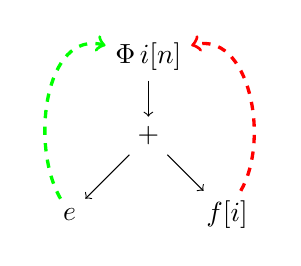
\begin{tikzpicture}
\node at (0, 2) (phi) {$\Phi\,i[n]$};
\node at (0, 1) (plus) {$+$};
\node at (-1, 0) (ee) {$e$};
\node at ( 1, 0) (eff) {$f[i]$};
\draw[->] (phi) -- (plus);
\draw[->] (plus) -- (ee);
\draw[->] (plus) -- (eff);
\draw[->, green, very thick, dashed] (ee) to [out=120,in=165] (phi);
\draw[->, red, very thick, dashed] (eff) to [out=60,in=15] (phi);
\end{tikzpicture}
  \caption{$f[i]$ cannot be moved outside $\phivec{i}{n}{e + f[i]}$, as it would \textit{skip} the binder of $i$ ($\Phi i[n]$) -- $e$ can be.}
\end{subfigure}
\caption{Example computations in common subexpression elimination (a) and loop-invariant code motion (b)}
\label{fig:transform-examples}
\end{figure}

\needspace{16em}
\subsection{Array-of-structs to struct-of-arrays}
\label{aos-to-soa}

A standard technique in compiling array programs is the array-of-structs (AoS) to struct-of-arrays (SoA) transformation \cite{shaikhha2019efficient}. The Ein compiler uses it to reduce all values to simple arrays of primitive types. This is crucial, as our compilation target -- NumPy,\footnote{Technically, NumPy does allow defining custom \texttt{dtype}s, but this feature is mostly intended for (de)serialising binary data. Similar features are nevertheless unavailable in other array libraries.} and array libraries generally -- lack support for arrays of composite types like pairs. Once we eliminate arrays of pairs, the only types $\tau'$ are given by:
\begin{align*}
\alpha &::= \kappa \mid \Box \alpha \\
\tau' &::= \alpha \mid \tau' \times \tau'
\end{align*}
Hence, $\tau'$ can only be tuples of arrays. This vastly simplifies compilation and runtime value representation. An AoS-to-SoA transformation is also applied in $\tilde F$ and Futhark, but it is not described in detail \cite{henriksen2017futhark, shaikhha2019efficient}. 

The isomorphism the operation relies on is $\Box (\tau_1 \times \tau_2) \cong \Box \tau_1 \times \Box \tau_2$, i.e. for each array of pairs there is an equivalent pair of arrays (of the same size). 
% As such, we need only consider the introduction and elimination forms of arrays of pairs. 
The core transformation is depicted in Figure \ref{fig:aos-to-soa}.
% We further aggressively eliminate intermediate pairs with rewrites given in Figure \ref{fig:pair-elim}.

\newcommand{\phisoa}[1]{\mathcal S \left\llbracket {#1} \right\rrbracket}
\newcommand{\phitupleindex}[2]{\mathcal P \left\llbracket {#1}, {#2} \right\rrbracket}

\begin{figure}
    \centering
    \begin{align*}
\phisoa {\phivec{i}{e_n}{e}}
&= \phipair{\phivec{i'}{\phisoa{e_n}}{\phifst{\phisoa{e}}}}{\phivec{i''}{\phisoa{e_n}}{\phisnd{\phisoa{e}}}}
&\text{(where }\Gamma; \Delta, i \vdash e : \phipairtype{\tau_1}{\tau_2} \text{)} \\[0.5em]
\phitupleindex{e}{e'}
&= \phipair{\phitupleindex{\phifst{e}}{e'}}{\phitupleindex{\phisnd{e}}{e'}}
&\text{(where }\Gamma; \Delta \vdash e : \phipairtype{\tau_1}{\tau_2} \text{)} \\
\phitupleindex{e}{e'}
&= e\left[ e' \right]
&\text{(where }\Gamma; \Delta \vdash e : \phivectype{\tau} \text{)} \\
\phisoa{e[e']}
&= \phitupleindex{\phisoa{e}}{\phisoa{e'}}
&\text{(where }\Gamma; \Delta \vdash e : \phivectype{\tau} \text{)} \\[0.5em]
\phisoa{e + e'}
&= \phisoa{e} + \phisoa{e'}
&\text{(and similarly for other cases)} \\[0.5em]
\phisoa{\phivectype{(\phipairtype{\tau_1}{\tau_2}})} &= \phipairtype{\phivectype{\tau_1}}{\phivectype{\tau_2}} &\text{(identity otherwise)}
    \end{align*}
$$ \phifst{\phipair{x}{-}} \leadsto x \quad \phisnd{\phipair{-}{y}} \leadsto y \quad \phipair{\phifst{p}}{\phisnd{p}} \leadsto p $$
    \caption{The core of the type-driven AoS-to-SoA transformation on Phi, denoted by $\mathcal S$. $\mathcal P$ maps an indexing to all arrays in the tuple. Environments $\Gamma; \Delta$ are passed through implicitly, in accordance with typing rules. It is succeeded by peephole optimisations which eliminate redundant pairs.}
    \label{fig:aos-to-soa}
\end{figure}

\needspace{5em}
\section{Escaping the Pointless with Axials}
\label{escaping-the-pointless}

\textbf{Axials} are the key contribution of this work. They establish a new formal connection from pointful to point-free array programming. Thus, we can escape programming pointless (point-free) code by translating pointful code to it. Their structure is natural, in the sense that it forms an applicative functor.


\newcommand{\sizeat}[1]{s_{#1}}
\newcommand{\altsizeat}[1]{S_{#1}}
\newcommand{\denotindex}{\mathrm{Index}}
\newcommand{\denotvalue}{\mathrm{Value}}
\newcommand{\denotvar}{\mathrm{Var}}
\newcommand{\denotenv}{\mathrm{Env}}
\newcommand{\denotenvindex}{\mathrm{IndexEnv}}
\newcommand{\denotenvvar}{\mathrm{VarEnv}}


\paragraph{Motivation}
We shall use $A \simeq B$ to denote an isomorphism, where there exist a bijection between sets $A$ and $B$. To motivate Axials, we appeal to the separation of identifiers in Phi into variables $x, y, z, \dots$ and indices $i, j, k, \dots$. Hence, there is a similar separation of environments $\denotenv \equiv (\denotvar + \denotindex) \to \denotvalue$:
$$ \denotenv \simeq \denotvar \times \denotenvindex $$
Let us now consider the denotation of a Phi expression $e$, given by $\llbracket e \rrbracket : \denotenv \to \denotvalue$. We can now apply currying within the denotation:
$$\llbracket e \rrbracket : \denotenv \to \denotvalue \simeq \denotenvvar \times \denotenvindex \to \denotvalue \simeq \denotenvvar \to \boxed{\denotenvindex \to \denotvalue}$$
Functions $\denotenvindex \to \denotvalue$ turn out to have a lot of structure.
Since indices are only introduced in  comprehensions, we know their values must be within a range of integers like $i \in \left[ 0, \sizeat i \right)$
-- where $\sizeat i$ is the \textit{size} of an index $i$, as introduced in $\phivec{i}{\sizeat i}{e}$. 
This leads us to say that:
$$ \mathrm{dom}\,\denotenvindex \simeq \left[0, \sizeat i \right) \times \left[0, \sizeat j \right) \times \left[0, \sizeat k \right) \times \dots $$ 
where $\iota = \{i, j, k, \dots \}$ are the free indices in $e$.%
\newcommand{\denotarrayiota}{\mathrm{Array}_{|\iota|}}
Indeed, thisx \textit{index space} directly corresponds to that of a $|\iota|$-dimensional array of shape $(\sizeat i, \sizeat j, \sizeat k, \dots)$ -- the set of which we denote $\denotarrayiota$. 
The difference is that our `array' has \textit{labelled} axes, rather than \textit{positional} ones.
We denote $\iota!$ as the set of permutations of $\iota$.\footnote{Throughout this text permutations are \textit{orderings} of a set -- sequences where each element occurs exactly once. If $\iota = \{i, j, k\}$, then $\iota! = \{[i, j, k], [i, k, j], [j, i, k], [j, k, i], [k, i, j], [k, j, i]\}$.}
To complete the connection with arrays, we need to order our labelled axes:
$$ \denotenvindex \to \denotvalue \simeq \iota! \to \denotarrayiota $$
We have obtained that expressions of type $\tau$ dependent on indices $\iota$ can be evaluated as a $|\iota|$-dimensional array of $\tau$. We shall assume onwards indices are \textit{intrinsically sized}, meaning we have a constant $s_i \in \mathbb N$.% 
\footnote{This is merely a useful assumption to clean up the rest of the reasoning. Note that in general there is a unique Phi \textit{expression} which computes the size -- and this is what the compilation scheme relies on.}

We can finally substitute the result back into the type of $\llbracket e \rrbracket$:
$$ \boxed{ \llbracket e \rrbracket : \denotenv \to \denotvalue \simeq \denotenvvar \to \iota! \to \denotarrayiota } $$
We took the jump from pointful \textit{(given an assignment to each index, compute $\tau$...)} to point-free style \textit{(using an array of values $\tau$ at each possible index...)}. \textbf{Axials} are an encoding of $\iota! \times \mathrm{Array}_{|\iota|}$, fixing the ordered \textit{axes} and encapsulating the connection on the point-free side. We define this encoding so that it is natural, and thus composes well from subexpressions of $e$.
% \footnote{For instance, if $e = e' + e''$, then the axial $\denot e$ can be given in terms of $\denot {e'}$ and $\denot {e''}$}

\paragraph{Definition} 
We define an Axial to be the type constructor $\mathrm{Axial}\,\alpha \equiv \mathrm{List}\,\mathrm{Index} \times \mathrm{Array}\,\alpha$. Elements of the list component are called the \textit{axes} (corresponding to $\iota!$ above), while the array is called the \textit{value} of the axial. We assume the rank of the value is the same as the number of axes; and each axis in the value has the same size as the index to which it corresponds.

We show Axials form an applicative functor. To this end, we need to define:\footnote{A complete proof would also show the definitions satisfy the \textit{applicative laws} (i.e. behave well under function composition).}
\begin{align*}
\mathrm{pure} &: \alpha \to \mathrm{Axial}\,\alpha \\
\mathrm{lift} &: (\alpha \to \beta \to \gamma) \to (\mathrm{Axial}\,\alpha \to \mathrm{Axial}\,\beta \to \mathrm{Axial}\,\gamma) 
\end{align*}
The former, $\mathrm{pure}$, is straightforward -- we can simply write:
$$ \mathrm{pure}\,a = \phipair{[]}{a} $$
On the other hand, to define $\mathrm{lift}\,f\,a\,b$, we need to think of an axial as a collection. We follow the formulation for $\mathrm{ZipList}$ (or a Naperian functor \cite{gibbons2016aplicative}), which applies $f$ elementwise to $a$ and $b$:
$$ \mathrm{lift}\,f\,a\,b \sim \Phi\, i.\, f(a[i], b[i]) $$
We need to perform a similar operation in a \textit{axis-aware} manner. The idea may be illustrated as follows. Say we have axials $a = \phipair{[i, j]}{\texttt{a}}$ and $b = \phipair{[k, j]}{\texttt{b}}$ . We want to unify their axes (free indices), producing an Axial $c = \phipair{\gamma}{\texttt{c}}$. We \textit{choose} the axes $\gamma = [i, j, k]$, in which case $\texttt{c}$ is given by:
$$ \texttt{c}[i, j, k] = f(\texttt{a}[i, j], \texttt{b}[k, j]) $$
this is essentially an instance of \textbf{broadcasting}, solidifying a connection with point-free array programming.

Without going into detail (the Axial setup is a bit different in the compilation scheme) and with some abuse of notation, we define the following $\mathrm{lift}$ for axials $a = \phipair{\alpha}{\texttt{a}}$ and $b = \phipair{\beta}{\texttt{b}}$:
$$ 
\mathrm{lift}\,f\,a\,b = \phipair{\gamma}{\Phi\,\overline{\gamma}. 
f \left( \texttt{a}[\overline{\gamma}]_\alpha^\gamma, \texttt{b}[\overline{\gamma}]_\beta^\gamma \right) } \quad \text{where } \gamma = \alpha \sqcup \beta
$$
where $\gamma = \alpha \sqcup \beta$ deterministically picks some permutation of axes from both $\alpha$ and $\beta$, and $\Phi\,\overline{\gamma}$ constructs a multidimensional array with indices in $\gamma$ (and sizes consistent with \texttt{a} and \texttt{b}). 
Indexing into $a$ and $b$ respects the new axes $\gamma$, removing and permuting indices.

% \paragraph{Examples} 
% Take $\mathrm{mergeAxes}\,x\,y = \mathrm{sort}\,(\mathrm{concat}\,x\,y)$. \\ Set $a = \{ [i, j], \{i \mapsto 2, j \mapsto 3 \}, [[0, 1, 2], [3, 4, 5]] \} $, $b = \{ [j, k], \{ j \mapsto 3, k \mapsto 1 \}, [[0], [-1], [-2]] \}$. Then:
% $$ d = \mathrm{lift}_2\,(+)\,a\,b = \{ [i,j,k], \{i \mapsto 2, j \mapsto 3, k \mapsto 1 \}, [[[0], [0], [0]], [[3], [3], [3]]] \} $$
% Similarly, set $c = \{ [j, i], \{ j \mapsto 3, i \mapsto 2 \}, [[0, -2], [1, -1], [2, 0]] \}$, in which case:
% $$ e = \mathrm{lift}_2\,(-)\,a\,c = \{ [i, j], \{i \mapsto 2, j \mapsto 3 \}, [[0, 0, 0], [5, 5, 5]] \} $$
% Note that $e[i, j] = a[i, j] - b[j, i]$, hence $e[1, 2] = a[1, 2] - b[2, 1] = 5 - 0 = 5$. 

% It is helpful to consider the examples in the context of Phi. In the first, $d$ is evaluating the outer $+$ in $$\phivec{i}{3}{\phivec{j}{2}{\phivec{k}{1}{(3 \cdot i + j) + (j + k)}}}$$ in terms of the sub-expressions $3 \cdot i + j$ and $j + k$ (with Axials $a$ and $b$ resp.). In the second one, $e$ is computing the result of the subtraction in 
% $$\phivec{i}{2}{\phivec{j}{3}{(3 \cdot i + j) - \mathrm{where}(i = 0, j, 2 - j)}}$$ again in terms of the subexpressions. $e[1, 2]$ corresponds to the substitution $\{ i \mapsto 1, j \mapsto 2 \}$:
% $$ e[1, 2] = (3 \cdot 1 + 2) - \mathrm{where}(1 = 0, 2, 2 - 2) = 5 - \mathrm{where}(\bot, 2, 0) = 5 - 0 = 5 $$

\paragraph{Context} Why are Axials useful in relating different styles of array programming? Crucially, instances of $\mathrm{lift}$ are essentially NumPy-style \textbf{broadcasting}.
In fact, Axials can be seen as a generalisation of arrays. 
Instead of \textit{positional axes}, we have a notion of \textit{labelled axes}. 
This is reminiscent of the recently introduced \textit{named tensors} \cite{chiang2022named}. 
% In-memory representation still requires us to pick the axis ordering.

It turns out Axials relate to two well-known applicative functors -- the $\mathrm{List}$ and $\mathrm{ZipList}$. 
So far, we did not specify $\denotindex$ beyond assuming it has a notion of equality. 
It turns out that under the right $\denotindex$ we obtain (roughly) the behaviour of existing applicatives.
When we take $\denotindex \equiv \mathrm{Unit}$ we obtain the $\mathrm{ZipList}$, for which $\mathrm{lift}$ always operates on lists elementwise.
% Any list can be converted to an Axial with the single axis, and $\mathrm{lift}\,f\,a\,b$ applies $f$ to respective pairs of elements in $a$ and $b$.
It is a well-known fact the $\mathrm{ZipList}$ cannot be generalised to a monad, thus there is no obvious Axial monad.
On the other hand, when $\denotindex \equiv \mathrm{Bool}$ we obtain the $\mathrm{List}$ applicative, for which $\mathrm{lift}$ operates on the cartesian product on lists. 
% For this construction, any application of $\mathrm{lift}$ needs to have the first operand along axis $\bot$, and the second along $\top$. 
% The result has both axes $\{ \bot, \top \}$, which we can convert back to a list by flattening -- thus applying $f$ for each pair in the cartesian product of $a$ and $b$.

\section{Code generation -- from pointful to point-free}
\label{codegen}

We now finally talk about how we can make the step from the pointful Phi calculus into the point-free array programming model. 
We devise \textit{Yarr} (a point-free array calculus), which is our target program representation. 
We show how Phi programs can be \textit{lifted} with the Axial, yielding a simple compilation scheme.

\subsection{Compilation target -- Yarr, the array calculus}
\label{yarr}

\begin{figure}
    \centering
    \begin{align*}
    \tau' ::=& \quad\kappa \mid \Box \tau' &\text{(arrays)} \\
    \tau ::=& \quad\tau' \quad\mid\quad \tau' \times \tau' \quad\mid\quad \dots &\text{(tuples of arrays)} \\
    E ::=&\quad \mathrm{range}(E)   &\text{(naturals up to }n\text{)} \\
    \mid&\quad \mathrm{size}(E, n)  &\text{(array size along axis)} \\
    \mid&\quad \mathrm{transpose}(E, (n, \dots)) &\text{(permute axes)} \\ 
    \mid&\quad \mathrm{squeeze}(E, n) &\text{(remove 1-axis)} \\
    \mid&\quad \mathrm{unsqueeze}(E, n) &\text{(add 1-axis)} \\
    \mid&\quad \mathrm{repeat}(E, E, n) &\text{(repeat along axis)} \\
    \mid&\quad \mathrm{gather}(E, E, n) &\text{(indexing along axis)} \\ 
    \mid&\quad \mathrm{elementwise}_\sigma(E, \dots) &\text{(elementwise op.)} \\
    \mid&\quad \langle E, \dots \rangle \quad\mid\quad \mathrm{proj}_n(E) &\text{(tuples and projections)} \\
    \mid&\quad \philet{x}{E}{E} &\text{(let-binding)} \\
    \mid&\quad \phifold{x}{E}{x}{E}{E} &\text{(indexed fold)} \\
    \mid&\quad x \quad\mid\quad c  &\text{(variables, constants)}
    \end{align*}
    \caption{The core of Yarr, our point-free array calculus. Operations are based on core NumPy primitives.}
    \label{fig:yarr-definition}
\end{figure}

We use a straightforward formalisation of point-free array programs for our compilation target, abstracting the interface of NumPy.
Figure \ref{fig:yarr-definition} shows the basic formulation into which we can compile Phi. It is extended with reductions, concatenation, specialised indexing operations (e.g. slicing), padding, and generalised Einstein summations. Note that the only significant common part with Phi is the indexed fold. In particular, indices $i$ from array comprehensions are erased entirely. The compilation scheme guarantees that no comprehension results in a fold. Otherwise, compiling Phi would be much easier -- one could set array elements one-by-one.

\needspace{5em}
\subsection{Compilation scheme}

\newcommand{\denot}[1]{\left\llbracket{#1}\right\rrbracket}

We now describe our scheme for compiling Phi into Yarr. It could be said it \textit{lifts} Phi expressions into the Axial applicative, at which point they are reified to computations in Yarr.

We introduce a transformation $\mathcal A \denot{e}$ mapping Phi terms $e$ to an Axial of Yarr terms $E$:
$$ \mathcal A \denot{e} = \langle \pi, E \rangle $$
where $\pi$ is a permutation of the free indices $\iota(e)$ of $e$. As with Axials, we call elements of $\pi$ the \textit{axes}. The encoding of $\mathcal A$ `flattens' the Axial \textit{values} -- and we set $\mathrm{rank}(E) = |\pi| + \mathrm{rank}(e)$. In part thanks to the fact Axials form an applicative, $\mathcal A \denot{e}$ can be composed from $\mathcal A$ for subterms of $e$. 

For a closed Phi program $p$, we shall expect that $P$ ($\mathcal A \denot{p} = \phipair{[]}{P}$) is its Yarr equivalent. It remains to fill in the gap where there are free indices, thus $\pi = \left[ \pi^{(1)}, \dots, \pi^{(k)} \right]$ is non-empty. We require the following \textit{semantic equivalence} property for $\mathcal A \denot e = \phipair{\pi}{E}$:
$$ \denot{\phivec{\pi^{(1)}}{\sizeat{\pi^{(1)}}}{\dots \phivec{\pi^{(k)}}{\sizeat{\pi^{(k)}}}{e}}} = \denot{E}$$
where $\sizeat i$ (in general, a Phi term) is used to denote the size of the range of index $i$. For example, consider $p = \phivec{i}{2}{\phivec{j}{3}{i + j}}$, so that $\sizeat i = 2$ and $\sizeat j = 3$. Then the following satisfies the property at $e \mapsto i + j$:
$$ \mathcal A \denot{i + j} = \phipair{[i, j]}{[[0, 1, 2], [1, 2, 3]]} $$

\newcommand{\sized}[1]{{#1} \triangleleft \sizeat{#1}}
We can now proceed to describe $\mathcal A$ for various Phi constructs. Firstly, we assumed that for any index $i$, we know the size $\sizeat i$. We achieve this by adding auxiliary Phi terms $\sized i$. Therefore:
$$ \mathcal A \denot{i \triangleleft \sizeat{i}} 
= \phipair{[i]}{ \mathrm{range} \left( \altsizeat{i} \right) }
\quad 
\text{where } \mathcal A \denot{\sizeat{i}} = \phipair{[]}{\altsizeat{i}} $$
To construct these auxiliaries, we substitute them at comprehensions (which introduce indices). Outside the comprehension body the index $i$ is no longer free, so we  remove $i$ from axes and adjust the encoding:
\newcommand{\dblsetminus}{\mathbin{{\setminus}\mspace{-5mu}{\setminus}}}
$$
\mathcal A \denot{\phivec{i}{\sizeat i}{e}} 
= \phipair{\mathcal \pi \dblsetminus i}{
\mathrm{transpose} \left( E, \theta_\pi^i \right)} 
\quad
\text{where } \mathcal A \denot{\{\sized i / i\} e} 
= \phipair{\pi}{E}
$$
where $\pi \dblsetminus i$ removes $i$ from $\pi$, and $\theta_\pi^i$ is the permutation that transposes the index $i$ onto the position of the outermost (Phi) axis. 
If $i$ was not free in $e$, we would use an appropriate $\mathrm{repeat}$ instead.

We now get to apply the Axial applicative. Constants $c$ are handled by $\mathrm{pure}\,c$ -- they have no axes:
$$ \mathcal A \denot{c} = \mathrm{pure}\,c $$
The other defining operation of an applicative -- $\mathrm{lift}$ -- also plays a central role. 
Take a scalar operator $e = \sigma(e_1, e_2)$, so that $\mathcal A \denot{e_1} = \phipair{\pi_{1}}{E_1}$ and $\mathcal A \denot{e_2} = \phipair{\pi_{2}}{E_2}$. 
We want to \textit{align} the results of $E_1$ and $E_2$ so that they have compatible axes $\pi$ which we can \textbf{broadcast} over. 
Indeed, $\pi$ needs to be a permutation of the indices $\iota(e_1) \cup \iota(e_2)$. 
This new choice of axes requires coercing $E_p$ ($p \in \{1, 2\}$) -- we need to first transpose $E_p$ (to match the order in $\pi$ from $\pi_{p}$), and then unsqueeze missing axes (the ones missing in $\pi_{p}$). 
We write $\pi = \mathrm{aligned}(\pi_{1}, \pi_{2})$ for choosing new axes, and the change-of-axes as $\mathrm{align}(E_p, \pi_{p}, \pi)$. The final formulation closely corresponds to a point-free $\mathrm{lift}\,\mathrm{elementwise}_\sigma$:
\begin{align*}
\begin{split}
&\pi = \mathrm{aligned}(\pi_{1}, \pi_{2}) \\
&E_1' = \mathrm{align}(E_1, \pi_{1}, \pi) \quad E_2' = \mathrm{align}(E_2, \pi_{2}, \pi) \\
&\mathcal A \denot{\sigma(e_1, e_2)} = \left\langle \pi, \mathrm{elementwise}_{\sigma}(E_1', E_2') \right\rangle 
\end{split}
% \tag{$\star$}
\end{align*}

We have covered the general technique on the core Phi constructs. We briefly overview the rest:
\begin{description}
    \item[Indexing] Indexing $e = e_1[e_2]$ is done in a very similar manner to elementwise operations, by synthesising a $\mathrm{gather}$ operator. The shape manipulation is a bit more involved -- general indexing is notoriously difficult to express in NumPy.
    \item[Folds] Folds are an interesting case. Both the accumulator and the body have axes which need to be aligned (same as before). Since iteration counts are independent of indices $i$, the fold step is perfectly data-parallel. Due to fold's generality, at runtime we interpret them as \mintinline{python}{for} loop -- but its overhead is often helped by data-parallelism.
    \item[Tuples] After the SoA-to-AoS transform (Section \ref{aos-to-soa}), we need only consider tuples of arrays of primitives. The encoding is generalised to support them by prepending axes $\pi$ to each array in the tuple.  
\end{description}
The Axial encoding is not unique due to the choice of \textit{axes} by $\mathrm{align}$. This choice has impact on performance -- it corresponds to the in-memory representation of the array. We use a deterministic heuristic to minimise the transpositions needed. 

% Compilation contract

\needspace{10em}
\section{Runtime -- Execution backends}
\label{execution-backend}

The compilation target of Ein is a high-level library in the array programming model. This means that most of the work is spent in large-workload whole-array operations, dominating the many overheads associated with Python. As such, we take some liberties to simplify the implementation. The primary technique we use is a (staging) function of the form
$$ \mathrm{Expr} \to \left( \denotenv \to \denotvalue \right) $$
where $\mathrm{Expr}$ is an expression in Phi or Yarr, and $\denotenv$ is a mapping from variables to assigned values. This essentially corresponds to directly implementing the denotational semantics $\llbracket e \rrbracket : \denotenv \to \denotvalue$ and composing the program from denotations of each subexpression $e$. We represent $\llbracket e \rrbracket$ with Python closures.

\subsection{Naive}

The first execution backend implemented was a \textit{na\"ive Phi interpreter}. It directly implements the denotational semantics of Phi, so Axial compilation is not necessary. 
% We still have to apply common subexpression elimination and loop-invariant code motion to avoid combinatorial explosion of the time complexity.
This backend was primarily used as a reference as time went on, as it was the easiest to extend. It focused on correctness rather than any notion of performance, and it is order of magnitudes slower than the NumPy backend. For example, staging $\phivec{i}{n}{2 \cdot i}$ results in a function \mintinline{python}{(dict[Variable, Value]) -> Value} equivalent to:
\begin{center}
\begin{cminted}{python}
lambda env: [2 * i for i in range(env[n])]
\end{cminted}
\end{center}

\subsection{NumPy}

We follow the same denotation-guided staging approach as in the naive backend. This time around we apply the whole suite of transformations and use Axial compilation from Phi to Yarr. The key difference is a stricter value representation that must rely on NumPy's \texttt{ndarray}s. We set values to be either arrays, or tuples of arrays. On this basis, we also apply some NumPy-specific performance optimisations.

\paragraph{Bindings} In some cases, NumPy attempts not to copy arrays, and instead returns a \textit{view}. For instance, \mintinline{python}{numpy.transpose(arr, (1, 0))} does not copy and instead returns an array with the same underlying data as \texttt{arr}, but a transposed layout. This is beneficial when the value is used once, but harmful when it is reused due to cache-inefficiency. We make use of a heuristic approach to address this -- whenever a view would be bound to a variable (hence reused), it is immediately copied to the target layout instead. 

Ein's let-bindings enjoy more efficient memory management than a manually-written NumPy program. In typical programs, new arrays are allocated sequentially. Afterwards, memory can only be freed by the garbage collector at the end of a function's scope. With explicit let bindings, we achieve higher granularity -- arrays can be freed as soon as they are no longer used.

\paragraph{Eliminating temporaries} Where they cannot return a view, NumPy operations allocate fresh memory for the result by default. Operations can be performed in-place instead, but idiomatic NumPy programs are inconvenient to write in this style (and thus waste memory). Consider adding three vectors \texttt{(a, b, c)}. The computation \texttt{a + b + c} will allocate memory for both \texttt{a + b} and \texttt{(a + b) + c}. If we can prove \texttt{a + b} will not be reused, we can reuse its memory. In NumPy, we would have to write:
\begin{center}
\begin{cminted}{python}
t = numpy.add(a, b)     # Allocate t = a + b
numpy.add(t, c, out=t)  # Reuse, update t := t + c
\end{cminted}
\end{center}
Ein's NumPy backend performs this in-place update optimisation automatically through a safe heuristic.
% which is more cache-friendly and saves needless memory allocations. 

\subsection{Generalising the NumPy backend}

The very same methods as in the NumPy can be used for other libraries -- such as PyTorch, TensorFlow, and Jax. This is because they all derive from NumPy, as explained in the Preparation chapter. A PyTorch backend was implemented to test this in practice. PyTorch can efficiently execute programs on hardware accelerators (like GPUs), since it implements a suite of well-optimised \textit{kernels}. This showcases a general principle -- existing libraries already implement hundreds of thousands of lines of performant code, and Ein can take advantage of this directly.

\paragraph{Automatic differentation} A feature common to all deep learning frameworks is the capability of performing \textit{automatic differentiation} (AD). Notably, we do not implement it directly in Ein. This choice is motivated by AD's availability in Ein's potential backends. Indeed, to differentiate an Ein function, we may use the PyTorch backend. In the following, we compute $\frac{\partial \mathbf{a}^T \mathbf{b}}{\partial \mathbf{a}} = \mathbf{b}$:
\begin{center}
\begin{cminted}{python}
import torch
# Initialise a pair of vectors with gradient tracking
a, b = (torch.randn(3).requires_grad_(True) for _ in range(2))
# Compute a dot product in Ein and execute in PyTorch
c = reduce_sum(lambda i: wrap(a)[i] * wrap(b)[i]).torch()
# Run backpropagation through Ein's torch graph
c.backward()
return a.grad  # == b
\end{cminted}
\end{center}

\paragraph{Abstract backend} To facilitate addition of new backends, the \texttt{AbstractArrayBackend} interface was implemented. It declares a standard set of array routines, from which a Yarr interpreter may be derived.

\subsection{Extrinsics}

There are cases where Ein's compiler does not directly generate calls to functions available in the backend. For instance, \texttt{numpy.sort} would never get called directly by Ein. To this end, \textit{extrinsics} were implemented to facilitate calls to backend-specific functions. This is facilitated with the \texttt{ext} primitive, which takes a function and its Ein type signature. Extrinsics allow nearly-seamless integration of Ein and custom code, which vastly improves flexibility. In the below example, we sort an Ein \mintinline{python}{Vec[Float]} using \texttt{numpy.sort}:
% (the \texttt{sort} wrapper is unnecessary, but used for clarity):
\begin{center}
\begin{cminted}{python}    
def sort(x: Vec[Float]) -> Vec[Float]:
    return ext(numpy.sort, ([Vec[Float]], Vec[Float]))(x)
a: Vec[Float] = wrap(numpy.array([2.5, 0.0, 1.0]))
return sort(a).numpy()  # [0.0, 1.0, 2.5]
\end{cminted}
\end{center}

Ein does have to make some assumptions about the provided function, forming the \textit{extrinsic contract}. Firstly, the function has to be pure -- it cannot mutate its arguments. Secondly, it has to be broadcastable over additional leading axes of the arguments. Lastly, the shape of the array returned by the extrinsic must only depend on the shape of the arguments, ensuring arrays remain rectangular. 
% CUT
% On the example of \texttt{numpy.sort}: it works on a copy of the array; when called on a matrix it sorts the columns of that matrix (its last axis), broadcasting over the first axis; and it always returns an array of the same shape as its argument.

\needspace{4em}
\section{Repository overview}
\label{repository-overview}

The Ein repository was built from scratch, and no pre-existing code was used.
It follows a usual Python project structure, with the root directory containing the \texttt{ein/} source directory, \texttt{tests/}, \texttt{tools/}, project configuration files (\texttt{pyproject.toml}, \texttt{.pre-commit-config.yaml}, etc.), and the Git configuration. 
A high-level breakdown is given in Table \ref{tab:repository}. The repository totals \todohere{} lines of Python code in the implementation and \todohere{} in the tests (as counted by \texttt{wc -l}, and the code formatted by \texttt{black}).

\begin{table}[h]
    \centering
    \begin{tabular}{c|c|l}
        Directory & Files & Description \\ \hline \hline
        \multirow{2}{*}{\texttt{ein/}} 
        & \texttt{debug.py} & Compiler debug utilities (e.g. \texttt{graphviz} diagrams) \\
        & \texttt{symbols.py}, \texttt{value.py}, \texttt{term.py} & Abstractions for defining Phi/Yarr \\ \hline
        \multirow{2}{*}{\texttt{ein/phi/}} & \texttt{phi.py} & Phi grammar and typing rules \\ 
        & \texttt{type\_system.py} & Type definitions \\ \hline
        \multirow{2}{*}{\texttt{ein/frontend/}} & \texttt{layout.py} & Encoding Ein records \\ 
        & \texttt{ndarray.py}, \texttt{comprehension.py}, \dots & Definitions of user-facing API \\ \hline
       \multirow{4}{*}{\texttt{ein/midend/}}       
        & \texttt{substitution.py} & Generic substitutions \\ 
        & \texttt{lining.py} & Inlining and outlining \\ 
        & \texttt{equiv.py}, \texttt{size\_classes.py} & Size equivalence judgements \\ 
        & \texttt{structs.py} & Array-of-structs to struct-of-arrays transform \\ \hline
       \multirow{3}{*}{\texttt{ein/codegen/}}       
        & \texttt{yarr.py} & Yarr grammar and typing rules \\ 
        & \texttt{axial.py} & Axials for Yarr \\ 
        & \texttt{phi\_to\_yarr.py}, \dots & Compilation scheme \\ \hline
       \multirow{3}{*}{\texttt{ein/backend/}}       
        & \texttt{naive.py} & Na\"ive Phi interpreter \\ 
        & \texttt{array\_backend.py} & Abstract array backend definition \\
        & \texttt{numpy\_backend.py} & Execution backends \\ \hline
       \texttt{tests/}       
        & \texttt{test\_*.py} & General and feature-specific tests \\ \hline 
       \texttt{tests/suite/}       
        & \makecell{\texttt{deep/*.py}, \texttt{misc/*.py}, \\ \texttt{parboil/*.py}, \texttt{rodinia/*.py}} & Longer programs \textit{(cases)} for tests and benchmarks \\ \hline 
       \texttt{tools/}
        & \texttt{benchmark.py} & Benchmarking utility \\ \hline 
        \texttt{.} & \texttt{pyproject.toml}, \dots & Project configuration files
    \end{tabular}
    \caption{Overview of the Ein repository.}
    \label{tab:repository}
\end{table}
